\scanpage{31}

\mspage{3}
is cocartesian -- or again, if $Y,X,X^*$
are connected, and we \unsure{choose|choose} a ``base point'' 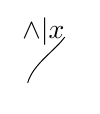
\begin{tikzpicture}[baseline=0pt,x=1cm,y=1cm]
\path[use as bounding box] (0,-.02) rectangle (.56,.72);
\draw[line width=.35pt] (0,.02) .. controls (.07,.26) and (.35,.43) .. (.47,.60);
\node[inner sep=0pt] at (.20,.67) {$\unsure{\wedge|x}$};
\end{tikzpicture} of $\Pi_1\mathcal V_{Y,X}^*$ (i.e. by definition, a universal covering of $\mathcal V_{Y,X}^*$) (hence \deleted{some}
base points of $\Pi_1\mathcal V_{Y,X}$, 
\begin{tikzpicture}[baseline=(old.base),x=1cm,y=1cm]
\node[anchor=base west,inner sep=0pt] (old) at (0,0) {\deleted{\unsure{and a point}}};
\node[anchor=base west,inner sep=0pt] at (-.18,.48) {\inserted{$\Pi_1X^*,\Pi_1X)$}};
\node[anchor=base west,inner sep=0pt] at (2.75,.40) {\deleted{of $\Pi_1X^*)$}};
\end{tikzpicture}, that we have a 
\begin{tikzpicture}[baseline=0pt,x=1cm,y=1cm]
\path[use as bounding box] (0,-.02) rectangle (1.20,.73);
\draw[line width=.35pt] (.02,.02) .. controls (.13,.22) and (.65,.34) .. (1.02,.40);
\node[anchor=base west,inner sep=0pt] at (.23,.49) {\inserted{canonical}};
\end{tikzpicture} isomorphism of funda-\\
mental groups

\[
(9)\qquad \Pi_1(X)\simeq\Pi_1(X^*)\wedge_{\Pi_1\mathcal V_{Y,X}^*}
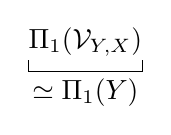
\begin{tikzpicture}[baseline=(v.base)]
\node[inner sep=0pt] (v) at (0,0) {$\Pi_1(\mathcal V_{Y,X})$};
\draw[line width=.35pt] ([yshift=-.04cm]v.south west) -- ([yshift=-.19cm]v.south west) -- ([yshift=-.19cm]v.south east) -- ([yshift=-.04cm]v.south east);
\node[anchor=north,inner sep=0pt] at ([yshift=-.27cm]v.south) {$\simeq\Pi_1(Y)$};
\end{tikzpicture},
\]

where $\Pi_1(\mathcal V_{Y,X})$ is isomorphic 
\begin{tikzpicture}[baseline=0pt,x=1cm,y=1cm]
\path[use as bounding box] (0,-.02) rectangle (2.95,.80);
\draw[line width=.35pt] (.02,.02) .. controls (.12,.27) and (.55,.36) .. (.95,.42);
\node[anchor=base west,inner sep=0pt] at (.22,.48) {\inserted{externall\textsuperscript{y}}};
\end{tikzpicture} to $\Pi_1(Y)$.

\deleted{\unsure{relative} to a chosen base point of}

To make $\Pi_1(X)$ explicit in terms of the
``elementary'' data, \deleted{it remains} including $\Pi_1(Y)$ 
\begin{tikzpicture}[baseline=0pt,x=1cm,y=1cm]
\path[use as bounding box] (0,-.02) rectangle (1.00,.65);
\node[anchor=base west,inner sep=0pt] at (.08,.37) {\inserted{and}};
\draw[line width=.35pt] (.02,.22) -- (1.00,.22);
\end{tikzpicture}
$\Pi_1(X^*)$, \unsure{\deleted{and}|and} it still 
\begin{tikzpicture}[baseline=(word.base),x=1cm,y=1cm]
\node[anchor=base west,inner sep=0pt] (word) at (0,0) {would remain};
\draw[line width=.35pt] (1.03,-.14) .. controls (1.00,.12) and (1.60,.24) .. (1.72,.52);
\end{tikzpicture} to make explicit the structure of $\Pi_1(\mathcal V_{Y,X}^*)$, which maps into the one and into the other, giving rise precisely to the diagram

\diagram{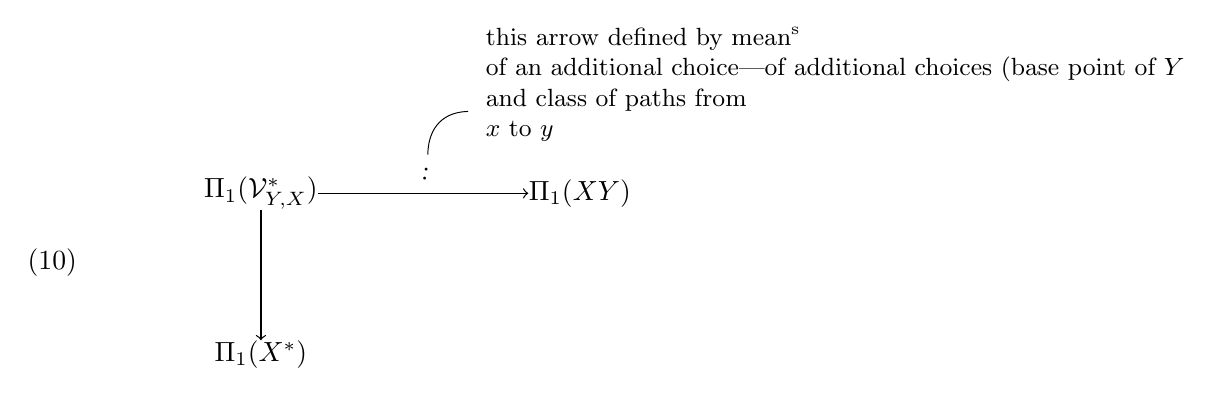
\begin{tikzpicture}[x=1cm,y=1cm]
\node[inner sep=0pt] at (-2.65,-.88) {$(10)$};
\node[inner sep=0pt] (a) at (0,0) {$\Pi_1(\mathcal V_{Y,X}^*)$};
\node[inner sep=0pt] (b) at (4.05,0) {$\Pi_1(\deleted{\unsure{X}}Y)$};
\node[inner sep=0pt] (c) at (0,-2.05) {$\Pi_1(X^*)$};
\draw[->,line width=.45pt] (a.east) -- (b.west);
\draw[->,line width=.45pt] (a.south) -- (c.north);
\node[anchor=south west,inner sep=0pt,align=left,font=\small] at (2.85,.65) {this arrow defined \unsure{by mean\textsuperscript{s}}\\
\unsure{of an additional choice|of additional choices} (base point of $Y$\\
and class of paths from\\
$x$ to $y$};
\draw[line width=.35pt] (2.63,1.04) .. controls (2.25,1.03) and (2.12,.76) .. (2.12,.49);
\node[inner sep=0pt] at (2.10,.29) {$\cdot$};
\node[inner sep=0pt] at (2.08,.18) {$\cdot$};
\end{tikzpicture}}

which expresses (8). It is here that the hypothesis

\margin{30}
